\documentclass[aspectratio=169,10pt]{beamer}
\usetheme{Madrid}
\usecolortheme{seahorse}
\setbeamertemplate{footline}[frame number]

\usepackage[utf8]{inputenc}
\usepackage{amsmath,amssymb,amsthm}
\usepackage{graphicx}
\usepackage{listings}
\usepackage{xcolor}
\usepackage{tikz}
\usetikzlibrary{arrows.meta,positioning,calc}

\graphicspath{{figures/}}

\lstset{
  basicstyle=\ttfamily\scriptsize,
  numbers=left,
  frame=single,
  backgroundcolor=\color{gray!7},
  keywordstyle=\color{blue}\bfseries,
  commentstyle=\color{green!50!black}\itshape,
  stringstyle=\color{red!60!black},
  breaklines=true,
  showstringspaces=false,
  language=Python
}

\newcommand{\B}{\mathbb{B}}
\newcommand{\N}{\mathbb{N}}
\newcommand{\R}{\mathbb{R}}
\newcommand{\Mcal}{\mathcal{M}}
\newcommand{\Msol}{\mathcal{M}_{sol}}
\newcommand{\Acal}{\mathcal{A}}
\newcommand{\Ecal}{\mathcal{E}}
\newcommand{\Hcal}{\mathcal{H}}
\newcommand{\Ocal}{\mathcal{O}}
\newcommand{\Rcal}{\mathcal{R}}

\title{Universal Artificial Intelligence}
\subtitle{Chapter 7}
\author{Chapter 7 --- Universal Artificial Intelligence}
\institute{An Introduction to Universal Artificial Intelligence \\ \small Hutter, Quarel, Catt (2024)}
\date{}

\begin{document}

% ============================================================
\begin{frame}
  \titlepage
  \vspace{-4mm}
  \begin{center}
  \small\itshape ``A sign of intelligence is an awareness of one's own ignorance.'' --- Niccol\`o Machiavelli
  \end{center}
\end{frame}

% ============================================================
\begin{frame}{Outline}
  \tableofcontents
\end{frame}

% ============================================================
\begin{frame}[allowframebreaks]{Recap: Agents, Environments, and Value (Chapter 6)}
  This chapter builds directly on the agent framework of Chapter 6, so we
  first recall the cast of characters. Everything here is about an
  \textbf{agent} that repeatedly picks an \textbf{action} and receives back
  a \textbf{percept} from the world, forever.

  \begin{itemize}
    \item \textbf{History} $h_{<t} = a_1e_1a_2e_2\dots a_{t-1}e_{t-1}$: the
      complete record of everything the agent has done and observed strictly
      before time $t$.
    \item \textbf{Percept} $e_t = (o_t,r_t)$: what the world hands back at
      time $t$ --- an observation $o_t$ together with a numerical reward
      $r_t\in[0,1]$.
    \item \textbf{Environment} $\nu$ (nu): a probability distribution
      $\nu(e_{1:t}\|a_{1:t})$ over percept sequences given the agent's
      action sequence --- i.e.\ the (possibly stochastic) rule the world
      uses to respond to actions. The double bar $\|$ marks this as a
      \emph{chronological semimeasure}: probabilities that only ever depend
      on the past, never the future.
    \item \textbf{True environment} $\mu$ (mu): whichever single $\nu$ is
      actually generating the agent's experience. In this chapter, whether
      $\mu$ is known or unknown to the agent is exactly what distinguishes
      the different agents we study.
    \item \textbf{Policy} $\pi$ (pi): the agent's strategy, a function from
      histories to a (possibly randomized) choice of next action.
    \item \textbf{Value function} $V_\nu^\pi(h_{<t})$: the total expected
      future discounted reward if the agent follows policy $\pi$ inside
      environment $\nu$, starting from history $h_{<t}$.
    \item \textbf{Discount function} $\gamma_k$ (gamma) and normalizer
      $\Gamma_t := \sum_{k=t}^\infty\gamma_k$: $\gamma_k$ is the weight
      placed on the reward received at future time $k$; discounting keeps
      the infinite sum of future rewards finite and expresses that sooner
      reward can matter more than later reward.
    \item \textbf{Q-value} $Q_\nu^\pi(h_{<t},a_t)$: the value of taking
      action $a_t$ right now and then following $\pi$ from then on.
    \item \textbf{Optimal value} $V_\nu^*(h_{<t}) := \max_\pi V_\nu^\pi(h_{<t})$
      and \textbf{optimal Q-value} $Q_\nu^*(h_{<t},a_t)$: the best possible
      value/Q-value achievable by \emph{any} policy in environment $\nu$.
  \end{itemize}

  \framebreak
  Chapter 6 defined $V$ and $Q$ generally, for \emph{any} choice of $\nu$ and
  $\pi$. This chapter is about specific, concrete choices of policy that try
  to actually maximize value, organized by how much the agent is told about
  the environment it is in:
  \begin{enumerate}
    \item \textbf{Section 7.1}: the environment $\mu$ is fully known
      $\Rightarrow$ agent \textbf{AI$\mu$}.
    \item \textbf{Section 7.2--7.3}: only a class $\Mcal$ of candidate
      environments is known, combined into a single Bayes mixture $\xi$
      (xi) $\Rightarrow$ agent \textbf{AI$\xi$}.
    \item \textbf{Section 7.4}: $\Mcal$ is taken to be \emph{every}
      computable environment, weighted by simplicity $\Rightarrow$ the
      universal agent \textbf{AIXI}.
  \end{enumerate}
\end{frame}

% ============================================================
\section{7.1 Acting Optimally in Known Environments}

\begin{frame}{Two Problems: Modelling and Planning}
  When an agent interacts with an environment to achieve its goals ---
  usually phrased as maximizing its value function --- there are two
  \emph{distinct} sub-problems:
  \begin{enumerate}
    \item \textbf{Modelling}: figuring out what the environment actually is.
    \item \textbf{Planning}: once the environment is known, figuring out
      the best way to act in it.
  \end{enumerate}
  If the agent is simply handed the true environment $\mu$ (mu), the
  modelling problem is ``solved'' by assumption\footnote{It could be that
  even when $\mu$ is given exactly, actually \emph{computing} with it is
  intractable --- but we set that concern aside in this section.}, leaving
  only the planning problem: choosing actions inside the known model $\mu$
  to maximize the value function. Replacing $\nu$ by the true environment
  $\mu$ in the general definitions of Chapter 6, and letting the lookahead
  horizon $m\to\infty$, gives our first concrete agent: the fully
  \textbf{informed optimal agent}, called \textbf{AI$\mu$}.
\end{frame}

% ============================================================
\begin{frame}{Definition 7.1.1: Policy of AI$\mu$}
  \begin{block}{Definition 7.1.1 (Policy of AI$\mu$)}
    Given the true environment $\mu$ and some discount function
    $\gamma_{(\cdot)}$, informed agent AI$\mu$ selects an optimal policy
    \[
      \pi_\mu^* \in \arg\max_\pi V_\mu^\pi \;\equiv\; \arg\max_\pi
      \lim_{m\to\infty} V_{\mu,\gamma}^{\pi,m}(\epsilon)
    \]
  \end{block}
  \textbf{Plain English.} $\pi_\mu^*$ (pi-mu-star) is \emph{any} policy that
  attains the maximum possible $\mu$-value: no other policy can do strictly
  better in environment $\mu$. The right-hand side spells this out as a
  limit: $V_{\mu,\gamma}^{\pi,m}(\epsilon)$ is the value obtainable by
  planning only $m$ steps ahead (starting from the empty history
  $\epsilon$), and we let the lookahead horizon $m$ grow to infinity so that
  no future reward, however far away, is ever left out of the calculation.
  AI$\mu$ (``AI-mu'') is thus the best conceivable agent \emph{given}
  perfect knowledge of the world it lives in --- it is the yardstick every
  other agent in this chapter will be measured against.
\end{frame}

% ============================================================
\begin{frame}[allowframebreaks]{Proposition 7.1.2: Action of AI$\mu$ (the Expectimax Tree)}
  \begin{block}{Proposition 7.1.2 (Action of AI$\mu$)}
    The action $a_t$ of AI$\mu$ at time $t$ given history $h_{<t}$ can be
    computed via
    \[
      a_t = a_t^{\mathrm{AI}\mu} := \arg\max_{a_t} Q_\mu^*(h_{<t},a_t)
    \]
    \[
      = \arg\max_{a_t}\lim_{m\to\infty}\sum_{e_t}\max_{a_{t+1}}\sum_{e_{t+1}}
      \dots \max_{a_m}\sum_{e_m}\prod_{k=t}^m\mu(e_k|h_{<k}a_k)
      \sum_{k=t}^m\gamma_k r_k
    \]
  \end{block}
  \textbf{Plain English, term by term.}
  \begin{itemize}
    \item $\arg\max_{a_t}(\cdot)$: the agent picks the action $a_t$ right
      now that leads to the best outcome.
    \item $\sum_{e_t}(\cdot)$: the environment then responds with some
      percept $e_t$, and since the agent does not control $e_t$, we average
      (sum) over all its possible values, weighted by how likely $\mu$ says
      each one is.
    \item $\max_{a_{t+1}}\sum_{e_{t+1}}\dots$: this max/sum pattern repeats,
      one time step at a time, out to the horizon $m$ --- the agent
      alternately \emph{chooses} (max) and the world \emph{responds}
      (weighted sum).
    \item $\prod_{k=t}^m\mu(e_k|h_{<k}a_k)$: the probability, under the true
      environment $\mu$, of the whole specific sequence of percepts along
      one particular branch of this decision tree.
    \item $\sum_{k=t}^m\gamma_k r_k$: the total discounted reward collected
      along that branch.
  \end{itemize}
  This alternating max/sum tree is called an \textbf{expectimax} tree ---
  exactly like a minimax game tree from game theory, except the adversary
  (``chance'') is replaced by nature's own probability distribution $\mu$.
\end{frame}

% ============================================================
\begin{frame}{Computing AI$\mu$ in Practice}
  \textit{Proof.} This follows immediately from Lemma 6.6.3 and Definition
  6.7.1 of Chapter 6, simply instantiated at $\nu=\mu$. $\blacksquare$

  \vspace{2mm}
  To directly compute $a_t^{\mathrm{AI}\mu}$ requires evaluating the
  expectimax tree truncated to an effective horizon
  $m = H_t(\varepsilon) < \infty$ (see Sections 6.7 and 12.1 for how large
  $\varepsilon$ (epsilon) must be to guarantee near-optimal behaviour). In
  practice, this is computationally expensive --- the tree has
  $|\Acal|^{m}\cdot|\Ecal|^m$ leaves, roughly --- so a variety of
  approximation techniques are used:
  \begin{itemize}
    \item \textbf{Pruning} or unrolling the expectimax calculation for only
      a short moving horizon.
    \item Using a hand-designed heuristic estimate $\widehat{Q}$ of the true
      $Q$-value in place of computing it exactly [RN20].
    \item Learning $\widehat{Q}$ from experience with a \textbf{neural
      network}, as in deep reinforcement learning systems.
    \item Approximating the expectimax with \textbf{Monte Carlo Tree
      Search (MCTS)}: several cheap \emph{rollouts} (playing the ``game''
      out to the end with a cheap proxy policy) are performed, and the
      resulting discounted sums of rewards are averaged to approximate the
      true expectation. This method is explored further in Section 12.2.2
      of the book.
  \end{itemize}
\end{frame}

% ============================================================
\begin{frame}[fragile]{Python: Expectimax Planning for AI$\mu$}
  \small Proposition 7.1.2 made concrete on a tiny \emph{known} 2-state
  environment: \texttt{hot} right after a reward of 1, \texttt{cold} right
  after a reward of 0; $\mu$ gives $P(\text{reward}=1\mid\text{state},a)$
  for each action $a\in\{0,1\}$ --- exactly what AI$\mu$ was built for.
  \begin{lstlisting}
# Known environment mu: P(reward=1 | state, action)
mu = {('hot',0): 0.5, ('hot',1): 0.8,
      ('cold',0): 0.5, ('cold',1): 0.3}
next_state = lambda r: 'hot' if r == 1 else 'cold'

def expectimax(state, steps_left):        # Prop. 7.1.2:
    if steps_left == 0:                   # max (agent) / sum (world)
        return 0.0, None
    best_a, best_v = None, -1.0
    for a in (0, 1):
        p1 = mu[(state, a)]               # mu(e_t=1|h,a)
        v = sum(p*(r + expectimax(next_state(r), steps_left-1)[0])
                for r, p in ((1, p1), (0, 1-p1)))   # sum over e_t
        if v > best_v: best_v, best_a = v, a        # max over a_t
    return best_v, best_a

for m in (1, 2, 3):
    v, a = expectimax('hot', m)
    print(f"horizon m={m}: V*_mu(hot)={v:.4f}, a_1={a}")
  \end{lstlisting}
  \textbf{Output:} \texttt{m=1: V*=0.8000, a\_1=1}, \ \texttt{m=2: V*=1.5400,
  a\_1=1}, \ \texttt{m=3: V*=2.2620, a\_1=1}. Even though action~1 only wins
  $80\%$ of the time in \texttt{hot}, it also \emph{keeps} the agent there
  more often than action~0, so it stays optimal at every horizon: expectimax
  correctly reasons several steps ahead, not just about immediate reward.
\end{frame}

% ============================================================
\section{7.2 Bayesian Mixture of Environments}

\begin{frame}{The Bayesian Solution to an Unknown Environment}
  In practice, the environment an agent interacts with is \emph{not} fully
  known. The classical reinforcement-learning fix is to make some (strong)
  assumption about the environment and then run some heuristic algorithm to
  learn it from the agent-environment interaction.

  \vspace{2mm}
  The \textbf{Bayesian} solution instead: consider a whole \emph{class}
  $\Mcal$ of candidate environments, large enough that we are confident it
  contains the true environment $\mu$; devise a prior weight $w_\nu$ for
  every $\nu\in\Mcal$; and use the known Bayes mixture $\xi$ (xi) in place
  of the unknown $\mu$. This mirrors exactly the sequence-prediction story
  of Chapter 3, now lifted to an agent that can also \emph{act}.
\end{frame}

% ============================================================
\begin{frame}{Definition 7.2.1: Chronological Bayes Mixture $\xi$}
  \begin{block}{Definition 7.2.1 (Chronological Bayes mixture $\xi$)}
    Let $\Mcal$ be a countable class of chronological semimeasures, and
    $w:\Mcal\to\R$ be a prior satisfying $\sum_{\nu\in\Mcal}w_\nu\le 1$ and
    $w_\nu>0$ for all $\nu\in\Mcal$. We define the \emph{chronological Bayes
    mixture} $\xi$ over $\Mcal$ given prior $w_{(\cdot)}$ as
    \[
      \xi(e_{1:t}\|a_{1:t}) := \sum_{\nu\in\Mcal} w_\nu\,\nu(e_{1:t}\|a_{1:t})
    \]
  \end{block}
  \textbf{Plain English.} $\xi$ is simply a weighted average of all the
  candidate environments in $\Mcal$, where each $\nu\in\Mcal$ contributes in
  proportion to its prior weight $w_\nu$ --- how plausible we thought $\nu$
  was \emph{before} seeing any data. Requiring $\sum_\nu w_\nu\le 1$ keeps
  $\xi$ itself a valid (chronological) semimeasure.

  \vspace{2mm}
  We will mainly restrict attention to countable policy spaces (e.g.\
  \emph{approximable} or \emph{limit-computable} policies, Definition
  2.6.13) rather than the uncountably many policies that exist in
  principle, since we are ultimately trying to build a physically
  realizable agent.
\end{frame}

% ============================================================
\begin{frame}{Definition 7.2.2: Bayesian Mixture as a Posterior}
  \begin{block}{Definition 7.2.2 (Bayesian mixture $\xi$ over environments)}
    Let $\Mcal$ be a class of environments with prior $\{w_\nu\}_{\nu\in\Mcal}$.
    We define $\xi(e_t|h_{<t}a_t)$ as the predictive probability the
    Bayesian mixture environment $\xi$ assigns to percept $e_t$ conditioned
    on history $h_{<t}$ and action $a_t$, recursively:
    \[
      \xi(e_t|h_{<t}a_t) := \sum_{\nu\in\Mcal} w(\nu|h_{<t})\,\nu(e_t|h_{<t}a_t)
    \]
    \[
      = \frac{\xi(e_{1:t}\|a_{1:t})}{\xi(e_{<t}\|a_{<t})}
      = \frac{\sum_{\nu\in\Mcal}w_\nu\,\nu(e_{1:t}\|a_{1:t})}
             {\sum_{\nu\in\Mcal}w_\nu\,\nu(e_{<t}\|a_{<t})},\quad\text{where}
    \]
    \[
      w(\nu|h_{1:t}) := w(\nu|h_{<t})\frac{\nu(e_t|h_{<t}a_t)}{\xi(e_t|h_{<t}a_t)}
      = w_\nu\frac{\nu(e_{1:t}\|a_{1:t})}{\xi(e_{1:t}\|a_{1:t})}
      \quad\text{and}\quad w(\nu|\epsilon):=w_\nu
    \]
  \end{block}
  \textbf{Plain English.} $w(\nu|h_{<t})$ is the agent's \emph{updated
  belief} that $\nu$ is the true environment, after seeing history
  $h_{<t}$; it starts at the prior $w_\nu$ and is refined by Bayes' rule
  every time a new percept arrives. This is exactly Theorem 3.1.7 from
  Chapter 3, but now every probability is additionally conditioned on the
  agent's own past actions $a_{<t}$ (and current action $a_t$), since here
  the ``agent'' actually gets to act rather than passively observe.
\end{frame}

% ============================================================
\begin{frame}[allowframebreaks]{Example 7.2.3: A Three-Coin Mixture Environment}
  \begin{block}{Example 7.2.3 (Mixture environment)}
    Consider a coin-flip prediction problem with $\Acal=\Ocal=\{H,T\}$,
    reward set $\{0,1\}$, and class
    $\Mcal=\{\nu_{HH},\nu_{HT},\nu_{TT}\}$ representing an environment that
    flips a two-headed coin, a fair coin, and a two-tailed coin,
    respectively. Each environment gives reward 1 to the agent if it
    correctly predicts the coin's outcome (i.e.\ if $a_t=o_t$). We choose
    the uniform prior $w_\nu=1/3$.
  \end{block}

  Initially the mixture predicts the likelihood of Heads is $1/2$:
  \[
    \xi(e_1{=}(H,1)|h_{<1}{=}\epsilon,a_1{=}H)
    = \sum_{\nu\in\Mcal} w_\nu\,\nu(e_1{=}(H,1)|a_1{=}H)
    = \tfrac13{\cdot}1 + \tfrac13{\cdot}\tfrac12 + \tfrac13{\cdot}0 = \tfrac12
  \]
  In fact, $\xi=\nu_{HT}$ exactly when the mixture is given an empty
  history --- the fair-coin environment and the mixture agree, since a
  $1/2$-$1/2$ mix of ``always Heads'' and ``always Tails'' looks just like a
  fair coin on the very first flip.

  \framebreak
  \textbf{The agent bets, and wins.} Suppose the agent takes action
  $a_1=H$ and guesses correctly, so the environment returns
  $(o_1,r_1)=(H,1)$, giving history $h_1=(a_1,e_1)=(H,(H,1))$. Applying the
  recursive update rule of Definition 7.2.2:
  \[
    w_{\nu_{HH}}(h_1) = \tfrac13\Big/\tfrac12 \cdot 1 = \tfrac23,\qquad
    w_{\nu_{HT}}(h_1) = \tfrac13\Big/\tfrac12 \cdot \tfrac12 = \tfrac13,\qquad
    w_{\nu_{TT}}(h_1) = \tfrac13\Big/\tfrac12 \cdot 0 = 0
  \]
  So the agent now believes with confidence $2/3$ that $\mu=\nu_{HH}$, with
  confidence $1/3$ that $\mu=\nu_{HT}$, and considers $\mu=\nu_{TT}$
  \emph{impossible} --- which makes sense, since a two-tailed coin could
  never have produced the observed Head.
  \begin{center}
  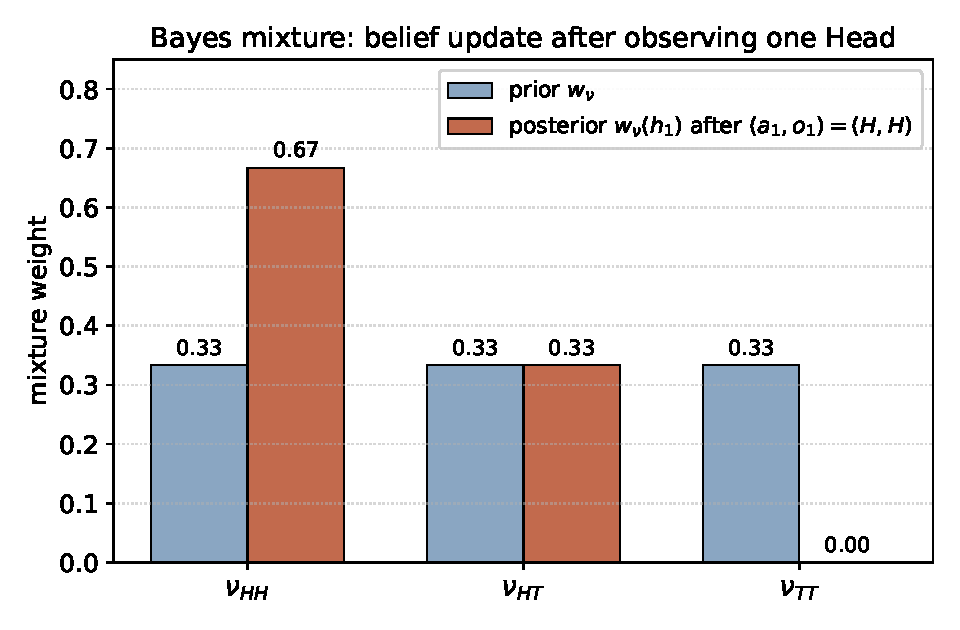
\includegraphics[width=0.55\textwidth]{mixture_weights}
  \end{center}

  \framebreak
  \textbf{Predicting further ahead.} Using the updated weights, the
  dynamics of $\xi(e_2|h_1a_2)$ become
  \[
    \xi(e_2|h_1a_2) = \sum_{\nu\in\Mcal}w(\nu|h_1)\nu(e_2|h_1a_2)
      = \tfrac23\nu_{HH}(e_2|h_1a_2) + \tfrac13\nu_{HT}(e_2|h_1a_2)
  \]
  and the probability that the next observation is Heads, for either choice
  of action $a_2$, is
  \[
    \xi(o_2{=}H|h_1H) = \tfrac23{\cdot}1+\tfrac13{\cdot}\tfrac12 = \tfrac56,
    \qquad
    \xi(o_2{=}H|h_1T) = \tfrac23{\cdot}1+\tfrac13{\cdot}\tfrac12 = \tfrac56
  \]
  In both cases $\xi$ predicts the next observation will be Heads with
  probability $5/6$, regardless of the action taken --- consistent with
  this being a \emph{passive} environment, where the agent's action only
  affects reward, not the coin. Note that $\xi\notin\Mcal$: the mixture
  itself is not one of the three original environments, which is expected
  given how limited this toy model class is. $\blacklozenge$
\end{frame}

% ============================================================
\begin{frame}[fragile]{Python: Reproducing the Coin-Mixture Example}
  \begin{lstlisting}
from fractions import Fraction as F

# nu[k] = P(outcome = H), for k in {HH, HT, TT}
nu = {'HH': F(1,1), 'HT': F(1,2), 'TT': F(0,1)}
w  = {k: F(1,3) for k in nu}              # uniform prior

# Agent bets a1=H, environment returns o1=H
like = {k: nu[k] for k in nu}
xi1 = sum(w[k]*like[k] for k in w)        # xi(o1=H|a1=H)
print("xi(o1=H|a1=H) =", xi1)             # -> 1/2

w_post = {k: w[k]*like[k]/xi1 for k in w}
for k in w_post:
    print(f"w_{k}(h1) =", w_post[k])
    # -> w_HH(h1)=2/3, w_HT(h1)=1/3, w_TT(h1)=0

xi2 = sum(w_post[k]*nu[k] for k in w_post)
print("xi(o2=H|h1) =", xi2)               # -> 5/6
  \end{lstlisting}
  Running this reproduces the book's numbers \emph{exactly} (using exact
  fractions rather than floating point): a prior of $1/3$ on each of the
  three coins collapses, after a single observed Head, to posterior weights
  $2/3, 1/3, 0$ --- and the mixture's prediction of the second flip being
  Heads rises to $5/6$.
\end{frame}

% ============================================================
\begin{frame}{Lemma 7.2.4: Linearity of the Posterior Mixture}
  \begin{block}{Lemma 7.2.4 (Linearity of posterior $\xi^\pi$ mixture)}
    For events $A\subseteq(\Acal\times\Ecal)^\infty$ and functions
    $f:(\Acal\times\Ecal)^\infty\to\R$,
    \[
      \mathrm{P}_\xi^\pi[A|h_{<t}] = \sum_{\nu\in\Mcal} w(\nu|h_{<t})\,
      \mathrm{P}_\nu^\pi[A|h_{<t}]
      \quad\text{and}\quad
      \mathbf{E}_\xi^\pi[f|h_{<t}] = \sum_{\nu\in\Mcal} w(\nu|h_{<t})\,
      \mathbf{E}_\nu^\pi[f|h_{<t}]
    \]
    Linearity with the same weights $w(\nu|h_{<t})$ remains true if we
    further condition on $a_t$. A particular instantiation is
    \[
      \xi^\pi(h_{1:m}) = \prod_{t=1}^m\pi(a_t|h_{<t})\nu(e_t|h_{<t}a_t)
      = \sum_{\nu\in\Mcal} w_\nu\,\nu^\pi(h_{1:m}) \;\ge\; w_\mu\,\mu^\pi(h_{1:m})
      \quad\forall\,\mu\in\Mcal
    \]
  \end{block}
  \textbf{Plain English.} Any probability or expectation computed under the
  mixture $\xi$, given a fixed policy $\pi$, is simply the corresponding
  probability/expectation under each individual $\nu$, averaged using the
  \emph{posterior} weights $w(\nu|h_{<t})$ --- exactly as one would hope
  from an average. The final inequality is the agent-case analogue of
  ``$\xi$ dominates every $w_\mu\mu$'' from Chapter 3: the mixture's
  probability of any full history is never smaller than any single
  environment's probability of it, scaled by that environment's prior
  weight.
\end{frame}

% ============================================================
\begin{frame}{Theorem 7.2.5: Linearity and Convexity of the Value Function}
  \begin{block}{Theorem 7.2.5 (Linearity/convexity of $V$)}
    $V_\nu^\pi(h_{<t})$ is linear in $\nu$ and $V_\xi^*(h_{<t})$ is convex
    in $\nu$:
    \[
      V_\xi^\pi(h_{<t}) = \sum_{\nu\in\Mcal} w(\nu|h_{<t})\,V_\nu^\pi(h_{<t})
      \qquad\text{and}\qquad
      V_\xi^*(h_{<t}) \le \sum_{\nu\in\Mcal} w(\nu|h_{<t})\,V_\nu^*(h_{<t})
    \]
    The same holds for the Q-values $Q_\nu^\pi(h_{<t}a_t)$ with the same
    weights $w(\nu|h_{<t})$.
  \end{block}
  \textbf{Plain English.} The \emph{fixed-policy} value $V^\pi$ behaves
  exactly like a weighted average (equality), because following one policy
  $\pi$ throughout is compatible with every $\nu$ simultaneously. But the
  \emph{optimal} value $V^*$ only satisfies an inequality ($\le$): on the
  left, one single policy $\pi_\mu^*$ must be tailored to $\mu$ alone; on
  the right, a single fixed policy must perform decently in \emph{every}
  $\nu\in\Mcal$ at once inside the mixture, which is a strictly harder ask,
  hence the mixture value can only be lower.
\end{frame}

% ============================================================
\begin{frame}{Theorem 7.2.6: Merging of Opinions}
  As $t\to\infty$ we would hope that $\xi\to\mu$ in a strong predictive
  sense, just as in Chapter 3's Corollary 3.3.2 (one-step predictive
  convergence). Two complications arise for an \emph{acting} agent: we now
  need \emph{multi-step} and \emph{off-policy} convergence, and discounted
  values require looking infinitely far ahead. It turns out this still
  holds, but without any guaranteed convergence \emph{rate}:
  \begin{block}{Theorem 7.2.6 (Merging of opinions [BD62])}
    \[
      \sup_A\big|\mathrm{P}_\xi^\pi[A|h_{<t}] - \mathrm{P}_\mu^\pi[A|h_{<t}]\big|
      \xrightarrow{t\to\infty} 0 \quad \mu^\pi\text{-a.s.}
    \]
    \[
      \sup_A\big|\mathrm{P}_\xi^\pi[A|h_{<t}a_t] - \mathrm{P}_\mu^\pi[A|h_{<t}a_t]\big|
      \xrightarrow{t\to\infty} 0 \quad \mu^\pi\text{-a.s.}
    \]
    where $\sup_A$ ranges over all measurable events
    $A\subseteq(\Acal\times\Ecal)^\infty$, and
    $\mathrm{P}_\nu^\pi[A|h_{<t}] = \mathbf{E}_\nu^\pi[\mathbb{1}_A|h_{<t}]$.
  \end{block}
  \textbf{Plain English.} No matter which \emph{measurable} question $A$ you
  ask about the entire infinite future, the mixture $\xi$'s answer and the
  true environment $\mu$'s answer eventually agree --- almost surely, when
  histories are sampled by running policy $\pi$ in the true environment
  $\mu$ (written $\mu^\pi$). Because this holds for \emph{every} such $A$
  simultaneously, it immediately implies both single-step convergence
  ($\xi(e_t|h_{<t}a_t)\to\mu(e_t|h_{<t}a_t)$) and $m$-step-ahead
  convergence for any fixed $m$. The figure a few slides ahead (after
  Theorem 7.3.6) plots this prediction gap shrinking towards $0$ in a small
  simulated example.
\end{frame}

% ============================================================
\section{7.3 Acting Optimally in Unknown Environments}

\begin{frame}{From Predictive Convergence to Value Convergence}
  Since $\xi\to\mu$ as $t\to\infty$ (Theorem 7.2.6), it is plausible to
  conjecture that the \emph{value function} $V_\xi$ also converges to
  $V_\mu$, regardless of which policy is used. Even if the agent always
  guessed the wrong action, it would still gather evidence about which
  environment it is really in, so it would eventually learn the truth
  anyway --- just without necessarily earning much reward while doing so.

  \vspace{2mm}
  \textbf{On-policy convergence.} If the agent actually follows a fixed
  policy $\pi$ while the true environment is $\mu$, then as $t\to\infty$ the
  computed value $V_\xi^\pi(h_{<t})$ converges to the true value
  $V_\mu^\pi(h_{<t})$ --- with probability 1 under $\mu^\pi$ (i.e.\ this
  failing has probability exactly zero).
\end{frame}

% ============================================================
\begin{frame}{Theorem 7.3.1: On-Policy Value Convergence of Bayes}
  \begin{block}{Theorem 7.3.1 (On-policy value convergence of Bayes)}
    For any environment $\mu\in\Mcal$ and any policy $\pi$,
    \[
      V_\xi^\pi(h_{<t}) - V_\mu^\pi(h_{<t}) \longrightarrow 0
      \quad\text{for } t\to\infty \quad \mu^\pi\text{-almost surely}
    \]
  \end{block}
  \textbf{Proof sketch.} Instantiate the general inequality
  \[
    \big|\mathbf{E}_Q[f]-\mathbf{E}_P[f]\big|
    \le \sup|f|\cdot\sup_A\big|Q[A]-P[A]\big|
  \]
  with $f=\sum_{k=t}^\infty\gamma_k r_k/\Gamma_t$ (the normalized future
  discounted reward), $P=\mathrm{P}_\mu^\pi(\cdot|h_{<t})$, and
  $Q=\mathrm{P}_\xi^\pi(\cdot|h_{<t})$. This gives
  \[
    \big|V_\xi^\pi(h_{<t}) - V_\mu^\pi(h_{<t})\big|
    \le \sup|f|\cdot\sup_A\big|\mathrm{P}_\xi^\pi[A|h_{<t}]-\mathrm{P}_\mu^\pi[A|h_{<t}]\big|
    \xrightarrow{t\to\infty} 0 \;\; \mu^\pi\text{-a.s.}
  \]
  The convergence follows since $\sup|f|\le\sup|\Rcal|\le1$ (rewards are
  bounded) and by Theorem 7.2.6 (merging of opinions). Convergence rates
  similar to, but weaker than, those of Chapter 3, Section 3.5, can also be
  obtained. $\blacksquare$
\end{frame}

% ============================================================
\begin{frame}{Definition 7.3.2: The Bayes-Optimal Agent AI$\xi$}
  We are ultimately interested in measuring an agent's performance against
  $V_\mu^*$, the optimal value function when $\mu$ is known and the best
  policy $\pi_\mu^*$ is used. Since $\mu$ is actually unknown, the best
  policy the agent \emph{can} choose is the one that maximizes its own best
  estimate $V_\xi^\pi$ of the environment, since $\xi$ represents the
  agent's best guess at $\mu$ given both the prior $w_\nu$ and everything
  observed so far.
  \begin{block}{Definition 7.3.2 (Bayes-optimal agent AI$\xi$)}
    \[
      \pi_\xi^* :\in \arg\max_\pi V_\xi^\pi
    \]
  \end{block}
  \textbf{Plain English.} AI$\xi$ (``AI-xi'') behaves exactly like AI$\mu$
  from Section 7.1, except it plans against its own current \emph{belief}
  $\xi$ about the world instead of the (unknown) true environment $\mu$.
  Representation Proposition 7.1.2 carries over unchanged with $\mu$
  replaced by $\xi$. Theorem 7.3.1 is reassuring, but it does \emph{not} yet
  tell us anything about how the value of \emph{this specific} policy
  $\pi_\xi^*$, evaluated in the true environment $\mu$, compares to the
  truly optimal value $V_\mu^*$.
\end{frame}

% ============================================================
\begin{frame}{Definition 7.3.3: Self-Optimizing Policies}
  What we really want to know is whether $V_\mu^{\pi_\xi^*}(h_{<t})$
  converges to $V_\mu^*(h_{<t})$ --- i.e.\ whether the true value achieved
  by the Bayes-optimal policy $\pi_\xi^*$ (the policy the agent actually
  has to use, in the face of an unknown $\mu$) converges to the value of the
  best policy $\pi_\mu^*$ it \emph{could} have used, had it known $\mu$ all
  along. In control theory this property is called \textbf{self-optimizing}:
  \begin{block}{Definition 7.3.3 (Self-optimizing policies)}
    A policy $\tilde\pi$ is called \emph{self-optimizing} for a class
    $\Mcal$ and historic policy $\pi$ if
    \[
      \forall\nu\in\Mcal:\quad V_\nu^*(h_{<t}) - V_\nu^{\tilde\pi}(h_{<t})
      \xrightarrow{t\to\infty} 0 \quad\text{with } \nu^\pi\text{ probability 1}
    \]
  \end{block}
  \textbf{Plain English.} $\tilde\pi$ (pi-tilde) eventually performs just as
  well as the best possible policy, \emph{in every single environment}
  $\nu\in\Mcal$ that could be the truth --- no matter which policy $\pi$ was
  used to generate the historic data $\tilde\pi$ is learning from. This is a
  strong, uniform requirement: while the future percepts $e_{1:\infty}$ are
  sampled from the real $\nu$, the \emph{past} actions $a_{<t}$ can be
  utterly arbitrary.
\end{frame}

% ============================================================
\begin{frame}{Lemma 7.3.4: Convergence of Posterior Averages}
  \begin{block}{Lemma 7.3.4 (Convergence of posterior averages [Lat23])}
    For any policy $\pi$, if $0\le\delta_{\nu,t}(h_{<t})\to0$ for
    $t\to\infty$ with $\nu^\pi$-probability 1, for all $\nu\in\Mcal$, then
    \[
      \sum_{\nu\in\Mcal} w_\nu\,\frac{\nu(e_{<t}\|a_{<t})}{\mu(e_{<t}\|a_{<t})}\,
      \delta_{\nu,t}(h_{<t}) \xrightarrow{t\to\infty} 0
      \quad\text{with } \mu^\pi\text{-probability 1}
    \]
    and equivalently
    $\displaystyle\sum_{\nu\in\Mcal} w(\nu|h_{<t})\,\delta_{\nu,t}(h_{<t})
    \xrightarrow{t\to\infty} 0$ with $\mu^\pi$-probability 1.
  \end{block}
  \textbf{Plain English.} $\delta_{\nu,t}$ (delta) is meant to represent a
  ``gap'' associated with environment $\nu$ at time $t$ that shrinks to zero
  for every individual $\nu$. This lemma says that a whole \emph{weighted
  average} of such gaps, weighted either by the likelihood ratio
  $\nu/\mu$ or (equivalently) by the posterior $w(\nu|h_{<t})$, also shrinks
  to zero --- a countable weighted sum of vanishing terms still vanishes,
  even though there are infinitely many terms and the weights themselves are
  changing over time. The proof (omitted here) uses that
  $X_t:=\nu(e_{<t}\|a_{<t})/\mu(e_{<t}\|a_{<t})$ forms a
  $\mu$-supermartingale, together with a reverse Fatou-lemma argument.
\end{frame}

% ============================================================
\begin{frame}[allowframebreaks]{Theorem 7.3.6: Self-Optimizing --- Statement and Proof}
  \begin{block}{Theorem 7.3.6 (Self-optimizing [Hut05b])}
    Let $\Mcal$ be a countable class of environments and $\pi$ be any
    historic policy. If there exists a self-optimizing policy $\tilde\pi$
    for $\Mcal$ in the sense of Definition 7.3.3, then the Bayes-optimal
    policy $\pi_\xi^*$ is self-optimizing for $\Mcal$.
  \end{block}
  \textbf{Why this matters.} This is one of the central results of the
  book. Obviously, if no self-optimizing $\tilde\pi$ exists at all, we
  cannot expect $\pi_\xi^*$ to be one either. So the sufficient condition
  here is also \emph{necessary} --- as weak an assumption as possible. Its
  strength compared to the asymptotic-optimality results of Chapter 8 is
  that it is \textbf{off-policy}: $\pi_\xi^*$ ends up self-optimizing even
  if the agent followed a completely different policy $\pi\ne\pi_\xi^*$ in
  the past.

  \framebreak
  \textbf{Proof.} For each $\nu\in\Mcal$ define
  $\delta_{\nu,t}(h_{<t}) := V_\nu^*(h_{<t}) - V_\nu^{\tilde\pi}(h_{<t})$.
  Since rewards are bounded by 1 and $V_\nu^*$ is a weighted average of
  rewards, $0\le V_\nu^{\tilde\pi}(h_{<t})\le V_\nu^*(h_{<t})\le r_{\max}=1$,
  which implies $0\le\delta_{\nu,t}\le1$. Additionally,
  \begin{align*}
    0 &\le w(\mu|h_{<t})\big[V_\mu^*(h_{<t}) - V_\mu^{\pi_\xi^*}(h_{<t})\big] \\
      &\le \sum_{\nu\in\Mcal} w(\nu|h_{<t})\big[V_\nu^*(h_{<t}) - V_\nu^{\pi_\xi^*}(h_{<t})\big] \\
      &\le \sum_{\nu\in\Mcal} w(\nu|h_{<t})\big[V_\nu^*(h_{<t}) - V_\nu^{\tilde\pi}(h_{<t})\big]
      = \sum_{\nu\in\Mcal} w(\nu|h_{<t})\,\delta_{\nu,t}(h_{<t})
  \end{align*}
  The first inequality holds because $V_\mu^*\ge V_\mu^{\pi_\xi^*}$ (the
  optimal value for $\mu$ is at least the value of any other policy). The
  second follows from adding only non-negative terms. The third follows
  because
  $\sum_\nu w(\nu|h_{<t})V_\nu^{\pi_\xi^*}(h_{<t}) = V_\xi^{\pi_\xi^*}(h_{<t})
  = V_\xi^*(h_{<t}) \ge V_\xi^{\tilde\pi}(h_{<t})
  = \sum_\nu w(\nu|h_{<t})V_\nu^{\tilde\pi}(h_{<t})$
  (Theorem 7.2.5, plus optimality of $\pi_\xi^*$ for $\xi$).

  \framebreak
  Dividing the chain of inequalities above by $w(\mu|h_{<t})$:
  \[
    0 \le V_\mu^*(h_{<t}) - V_\mu^{\pi_\xi^*}(h_{<t})
    \le \frac{1}{w_\mu}\sum_{\nu\in\Mcal}w_\nu\,
    \frac{\nu(e_{<t}\|a_{<t})}{\mu(e_{<t}\|a_{<t})}\,\delta_{\nu,t}(h_{<t})
  \]
  which by Lemma 7.3.4 converges to $0$ as $t\to\infty$ with
  $\mu^\pi$-probability 1. Since this holds for every $\mu\in\Mcal$,
  $\pi_\xi^*$ is self-optimizing. $\blacksquare$
\end{frame}

% ============================================================
\begin{frame}{Figure 7.1: Which Environment Classes Admit Self-Optimizing Agents?}
  \centering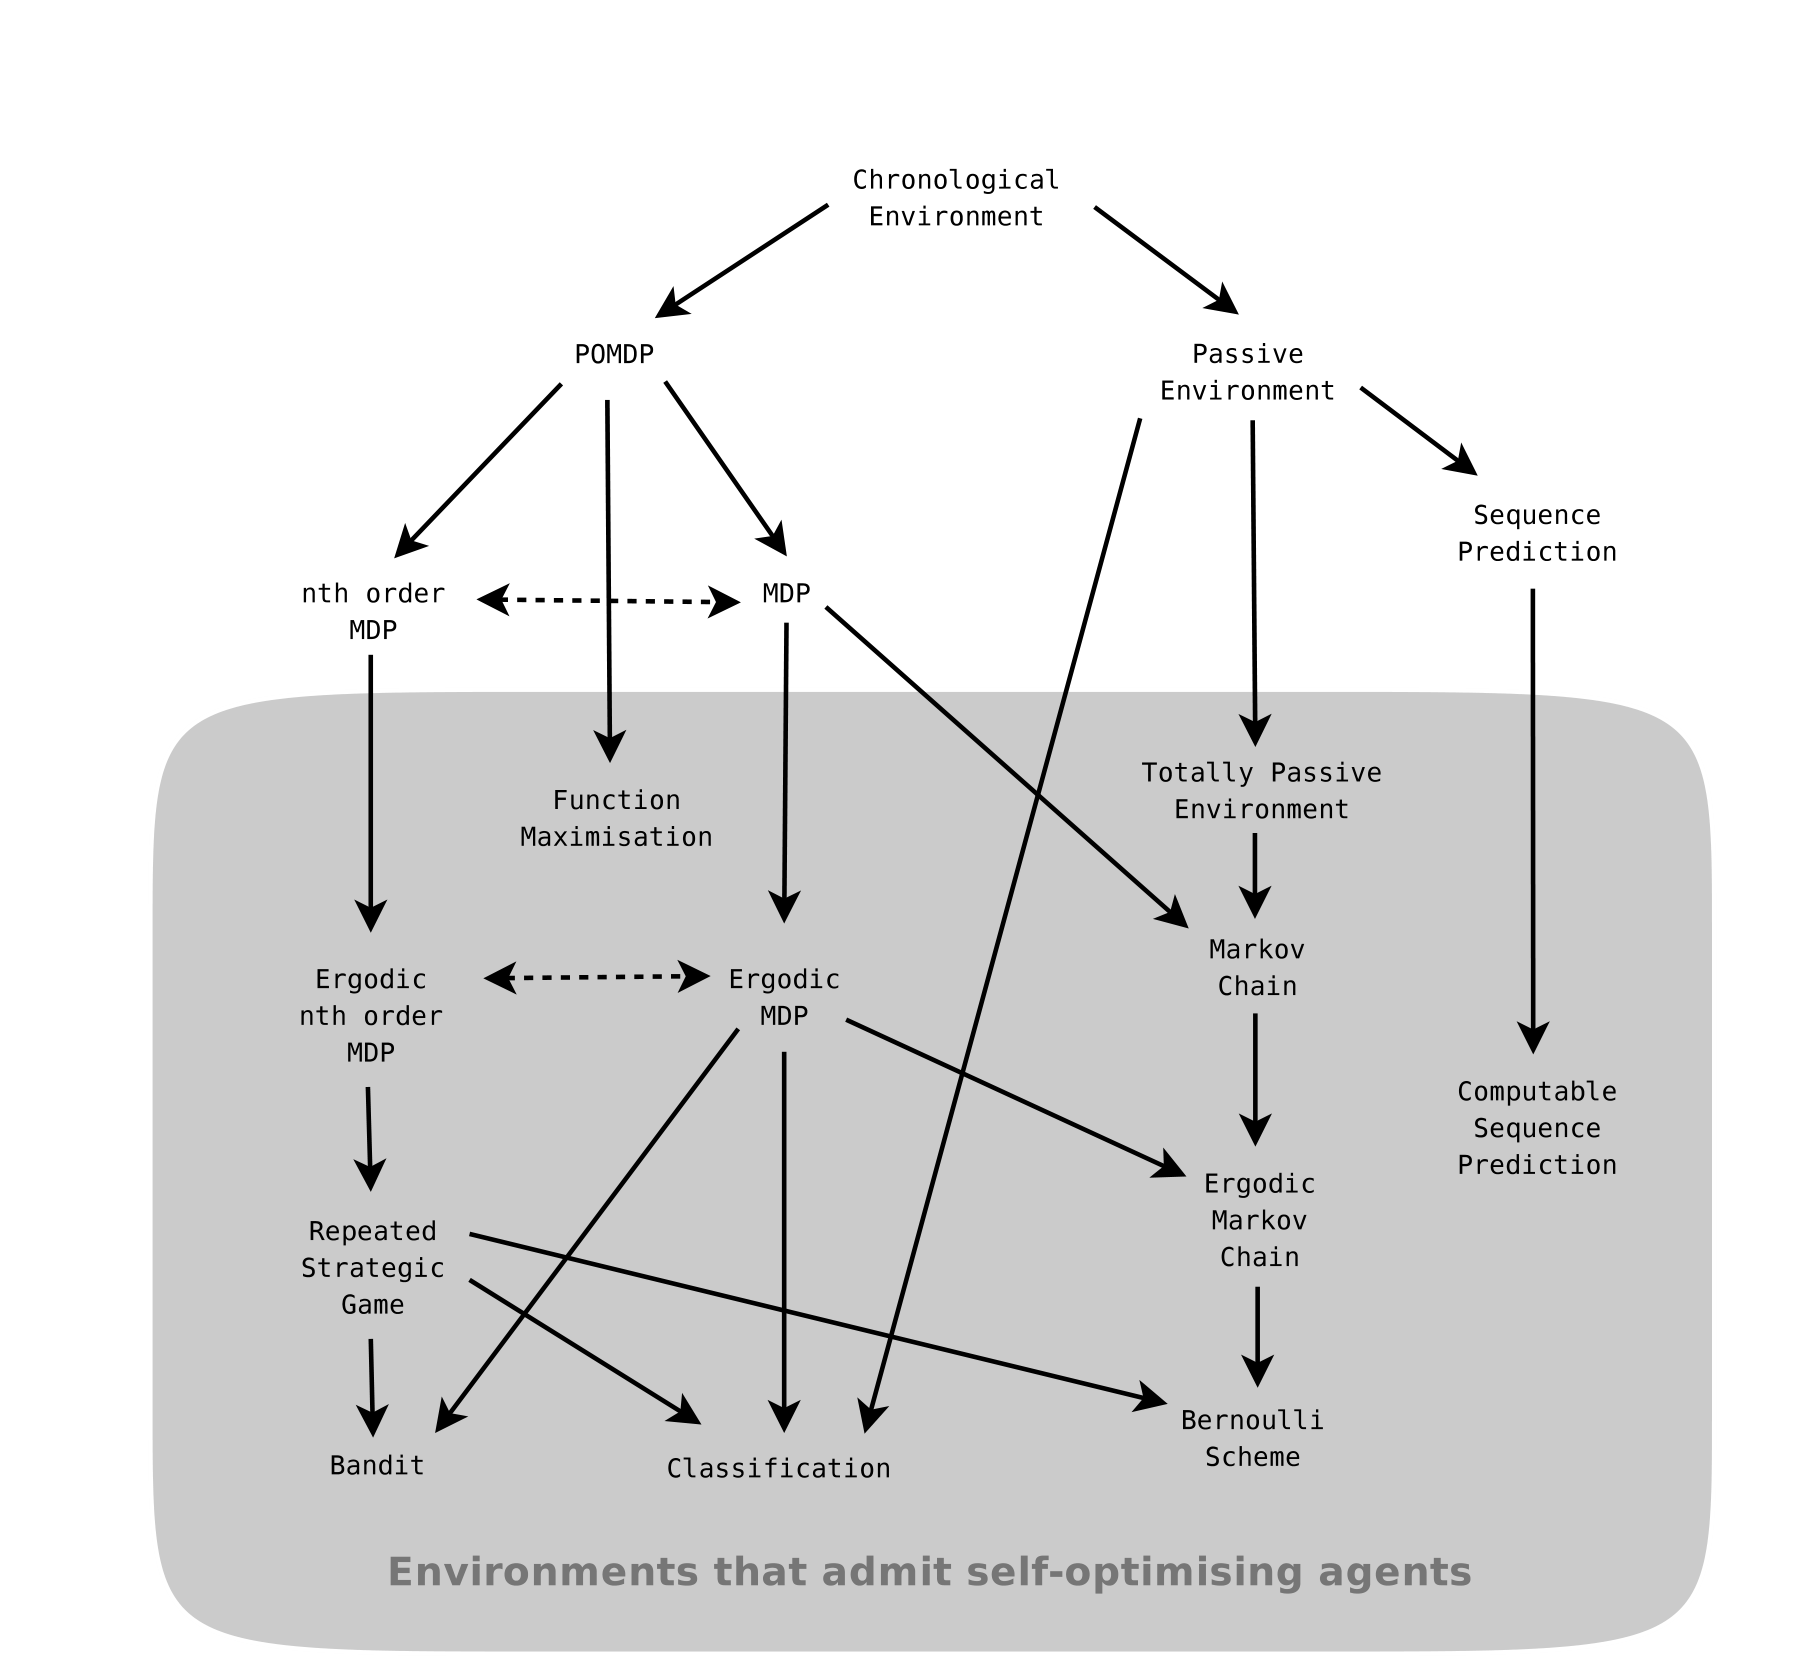
\includegraphics[width=0.46\textwidth]{taxonomy}
\end{frame}

% ============================================================
\begin{frame}{Reading the Taxonomy}
  Downward arrows in Figure 7.1 (previous slide) mean ``the class below is a
  special case of the class above.'' Dotted horizontal lines mean two
  classes are \emph{reducible} to each other. The \textbf{grey region}
  contains exactly the environment classes that \emph{do} admit
  self-optimizing agents --- ergodic $n$th-order MDPs (Markov Decision
  Processes) are one large such class, hence $\pi_\xi^*$ is self-optimizing
  for them by Theorem 7.3.6. Sequence prediction is Chapter 3's topic;
  Markov chains, Chapters 4--5; (ergodic) $n$th-order MDPs, Chapters 11,
  12, 14.
\end{frame}

% ============================================================
\begin{frame}{Self-Optimizing Fails Without Ergodicity: Traps}
  Unfortunately, \emph{without} some form of \textbf{ergodicity}
  assumption --- roughly, the requirement that the agent can always find its
  way back to explore any part of the environment again --- self-optimizing
  fails, because the agent can fall into \textbf{traps}: parts of the state
  space from which it can never recover, so early mistakes become
  permanent. The book's ``Heaven-Hell'' example (Example 8.1.3, covered in
  Chapter 8) illustrates this concretely: one wrong early action locks the
  agent forever into a low-reward region it can never escape.

  \vspace{2mm}
  \textbf{Consequence.} The class of \emph{all} (semi)computable
  chronological environments --- with no ergodicity restriction --- does
  \textbf{not} admit self-optimizing policies. This is exactly the gap that
  motivates weaker, \emph{on-average} notions of optimality, which Chapter
  8 develops.
\end{frame}

% ============================================================
\begin{frame}{Convergence in Practice: Merging of Opinions and Self-Optimizing}
  \small The two theorems of this section --- merging of opinions
  (Thm.\ 7.2.6) and self-optimizing (Thm.\ 7.3.6) --- both describe
  quantities shrinking to $0$ over time, simulated below on a small
  three-environment Bernoulli mixture (uniform prior) acting greedily in a
  fixed true environment $\mu$.
  \begin{center}
  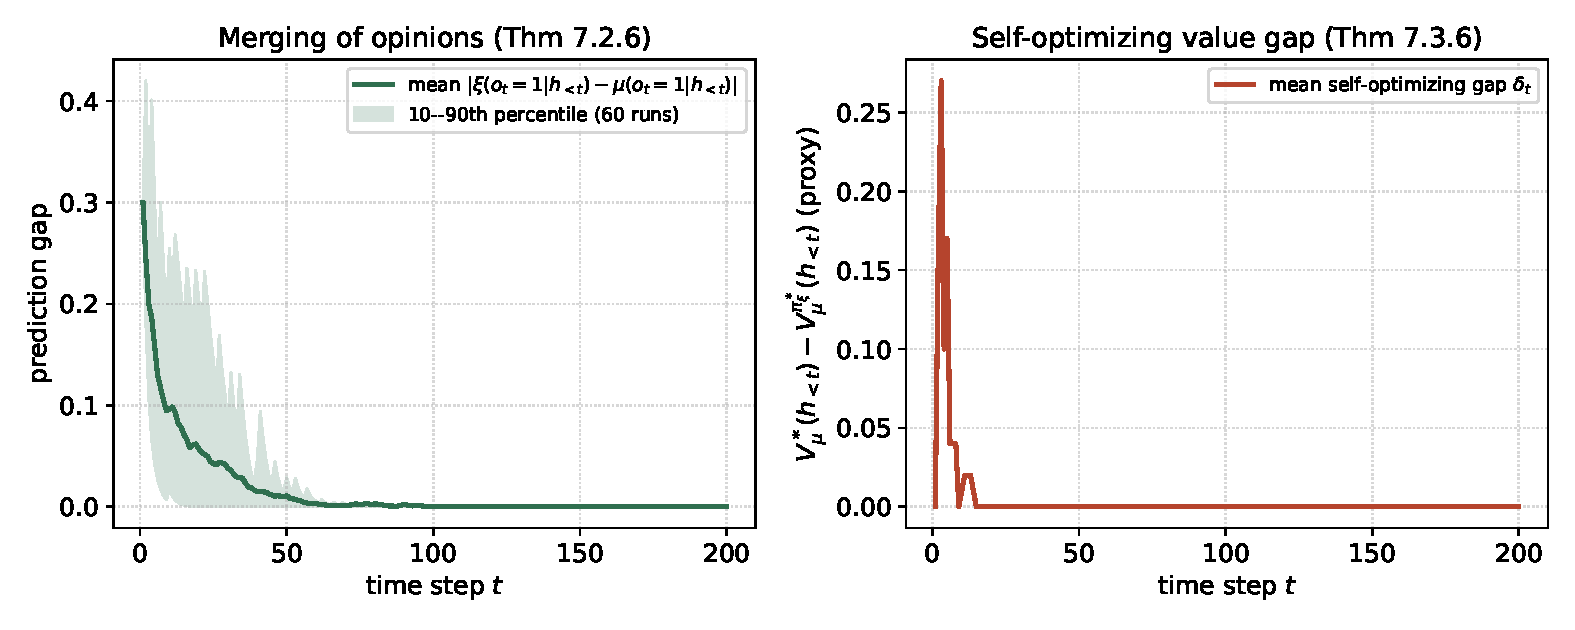
\includegraphics[width=0.78\textwidth]{convergence}
  \end{center}
  \small\textbf{Left:} the prediction gap
  $|\xi(o_t{=}1|h_{<t})-\mu(o_t{=}1|h_{<t})|$ (Thm.\ 7.2.6). \textbf{Right:}
  the self-optimizing value gap
  $\delta_t=V_\mu^*(h_{<t})-V_\mu^{\pi_\xi^*}(h_{<t})$ (Thm.\ 7.3.6). Both
  shrink towards $0$ once the mixture is confident which environment it
  faces.
\end{frame}

% ============================================================
\section{7.4 Universal Optimal Agent AIXI}

\begin{frame}{From AI$\xi$ to AIXI: the Universal Mixture}
  So far we have considered a \emph{general} environment class $\Mcal$ and a
  \emph{general} prior $w_\nu$. We can now combine our earlier choice of
  class and prior (motivated by Occam's razor and Epicurus' principle of
  multiple explanations, Section 3.7) with the notion of a Bayesian agent,
  arriving at the \textbf{universal Bayesian agent AIXI}.

  \vspace{2mm}
  AI$\xi$ from the previous section is exactly like AI$\mu$, except it does
  not know the true environment, so we replaced $\mu$ with $\xi$, the
  Bayesian mixture over $\Mcal$. We now define \textbf{AIXI} to be the
  universal Bayesian agent that uses the class of \emph{all}
  lower-semicomputable chronological semimeasures $\Mcal=\Msol$, together
  with the \textbf{universal prior} $w_\nu = w_\nu^U := 2^{-K(\nu)}$ and
  mixture distribution $\xi=\xi_U$. Here $K(\nu)$ is the \textbf{Kolmogorov
  complexity} of $\nu$ --- the length, in bits, of the shortest computer
  program that computes $\nu$ --- so simpler (shorter-description)
  environments get exponentially more prior weight: Occam's razor, made
  precise.
\end{frame}

% ============================================================
\begin{frame}{Definition 7.4.1: The Universal Optimal Agent AIXI}
  \begin{block}{Definition 7.4.1 (Universal optimal agent AIXI)}
    AIXI is the Bayes-optimal agent for the universal mixture
    $\xi_U(\cdot) := \sum_{\nu\in\Msol} w_\nu^U\,\nu(\cdot)$, with universal
    prior $w_\nu^U := 2^{-K(\nu)}$:
    \[
      \pi^{\mathrm{AIXI}} := \pi_{\xi_U}^* = \arg\max_\pi V_{\xi_U}^\pi
    \]
  \end{block}
  \textbf{Plain English.} AIXI is precisely AI$\xi$ from Section 7.3, with
  the class $\Mcal$ specialized to \emph{every computable environment} and
  the prior specialized to the \emph{universal prior} $2^{-K(\nu)}$. There
  is no further tuning knob left to choose: this is the most
  environment-independent Bayesian agent conceivable.

  \vspace{2mm}
  AIXI is regarded as the most ``intelligent'' environment-independent agent
  possible because it optimally learns and acts across an enormous range of
  environments, adapts to whatever situation it finds itself in, and
  combines all hypotheses according to Occam's razor. As it interacts with
  its environment, it continuously updates its beliefs $w(\nu|h_{<t})$,
  gathering more information over time and refining its understanding,
  which lets it make progressively better-informed decisions.
\end{frame}

% ============================================================
\begin{frame}{Theorem 7.4.2: Expectimax Bayesian Form of AIXI}
  \begin{block}{Theorem 7.4.2 (Expectimax Bayesian form of AIXI)}
    For finite lifetime $m$ and no discounting, i.e.\
    $\gamma_k=\mathbb{1}[k\le m]$, given interaction history $h_{<t}$, the
    action of AIXI at time $t$ has the explicit expectimax expression
    \[
      a_t = \pi_{\xi_U}^*(h_{<t}) = \arg\max_{a_t}\sum_{e_t}\max_{a_{t+1}}
      \sum_{e_{t+1}}\dots\max_{a_m}\sum_{e_m}\Big[\sum_{i=t}^m r_i\Big]
      \sum_{\nu\in\Msol} w_\nu^U(h_{<t})\prod_{k=t}^m\nu(e_k|h_{<k}a_k)
    \]
    where $w_\nu^U(h_{<t})$ is the posterior (Definition 7.2.2) for
    universal prior $w_\nu^U(\epsilon):=2^{-K(\nu)}$.
  \end{block}
  \textbf{Plain English.} $\mathbb{1}[k\le m]$ (the indicator function) is 1
  for $k\le m$ and 0 otherwise: rewards count in full up to the fixed
  horizon $m$ and not at all beyond it --- ``no discounting'' up to a
  cutoff. Everything else is the same expectimax alternation as
  Proposition 7.1.2, except the single known $\mu$ has been replaced by an
  explicit sum over the \emph{entire} universal class $\Msol$, each term
  weighted by the current posterior belief $w_\nu^U(h_{<t})$ in that
  environment.
\end{frame}

% ============================================================
\begin{frame}{Proof of Theorem 7.4.2}
  \textit{Proof.} The explicit expression for the action
  $a_t=\pi_\nu^*(h_{<t})$ of AI$\nu$ was given in Chapter 6 (Eq.\ 6.7.7).
  Replacing $\nu$ by $\xi$ gives AI$\xi$. The key step is rewriting the
  product of $\xi$-probabilities purely in terms of the individual $\nu$'s:
  \[
    \prod_{k=t}^m\xi(e_k|h_{<k}a_k)
    = \frac{\xi(e_{1:m}\|a_{1:m})}{\xi(e_{<t}\|a_{<t})}
    = \frac{\sum_\nu w_\nu\,\nu(e_{1:m}\|a_{1:m})}{\xi(e_{<t}\|a_{<t})}
  \]
  \[
    = \sum_\nu w_\nu\,\frac{\nu(e_{<t}\|a_{<t})}{\xi(e_{<t}\|a_{<t})}
    \prod_{k=t}^m\nu(e_k|h_{<k}a_k)
    = \sum_\nu w(\nu|h_{<t})\prod_{k=t}^m\nu(e_k|h_{<k}a_k) \tag{7.4.3}
  \]
  where we used Definitions 7.2.1 and 7.2.2 twice. AIXI is simply the
  special case for $\Msol$, $w_\nu^U$, and $\xi_U$, which proves the
  theorem. $\blacksquare$

  \vspace{2mm}
  There is yet another --- arguably the most elegant --- formulation of
  AIXI, based on a variant of the monotone Turing machine, which we define
  next.
\end{frame}

% ============================================================
\begin{frame}{Definition 7.4.4: Chronological Turing Machine}
  \begin{block}{Definition 7.4.4 (Chronological Turing machine)}
    A (monotone) Turing machine $T$ is called a \emph{chronological Turing
    machine} if, when fed a program $p$, it transforms an input data stream
    $a_{1:m}$ into an output data stream $e_{1:m}$ such that for all
    $k\le m$, it must print each ``percept'' $e_k$ on the output tape prior
    to reading the next ``action'' $a_{k+1}$ from the input tape. Formally
    $p'$, $a_k$, $o_k$, $r_k$, $e_k\equiv o_kr_k$ are all understood to be
    encoded prefix-free, so that they can be uniquely decoded from $a_{1:m}$
    and $e_{1:m}$. Notationally we define
    \[
      T(p'a_{1:m})\to e_{1:m} \text{ is true} \quad\text{iff}\quad
      T(p'a_{1:k}) = e_{1:k} \text{ for all } k\le m
    \]
  \end{block}
  \textbf{Plain English.} This is just a careful bookkeeping device: it
  formalizes the ``chronological'' requirement (percepts printed before the
  next action is read) inside a program that can also read inputs
  \emph{interactively}, so we can talk rigorously about a Turing machine
  that plays the role of an agent's ``model'' of the environment while
  respecting the actual time ordering of the interaction.
\end{frame}

% ============================================================
\begin{frame}{Theorem 7.4.5: Expectimax Solomonoff Form of AIXI}
  \begin{block}{Theorem 7.4.5 (Expectimax Solomonoff form of AIXI)}
    The action of undiscounted horizon-$m$ AIXI at time $t$ given
    interaction history $h_{<t}$ is:
    \[
      a_t^* = \pi_M^*(h_{<t}) = \arg\max_{a_t}\sum_{e_t}\dots\max_{a_m}
      \sum_{e_m}\big[r_t+\dots+r_m\big]\,M(e_{1:m}\|a_{1:m})
    \]
    where
    \[
      M(e_{1:m}\|a_{1:m}) := \sum_{p\,:\,U(p'a_{1:m})\to e_{1:m}} 2^{-\ell(p)}
    \]
    is a chronological version (Definition 6.3.1) of Solomonoff's
    distribution (3.8.3), and $U$ is a chronological Universal Turing
    machine (Definition 7.4.4).
  \end{block}
  \textbf{Plain English.} $\ell(p)$ is the length, in bits, of program $p$.
  $M$ sums $2^{-\ell(p)}$ over \emph{every} program $p$ that, when combined
  with the agent's action tape $a_{1:m}$, causes the universal machine $U$
  to output exactly the percept sequence $e_{1:m}$: shorter programs
  contribute exponentially more weight, so this is a direct algorithmic
  (program-length-based) restatement of the same universal-prior idea, this
  time phrased over programs rather than over environments.
\end{frame}

% ============================================================
\begin{frame}{Proof of Theorem 7.4.5: Equivalence with the Bayesian Form}
  \textit{Proof.} The inner sum of Theorem 7.4.2 can be written as
  \[
    \sum_{\nu\in\Mcal} w(\nu|h_{<t})\prod_{k=t}^m\nu(e_k|h_{<k}a_k)
    = \frac{\xi(e_{1:m}\|a_{1:m})}{\xi(e_{<t}\|a_{<t})} \tag{7.4.6}
  \]
  where $\xi(e_{1:m}\|a_{1:m}):=\sum_{\nu\in\Mcal}w_\nu\,\nu(e_{1:m}\|a_{1:m})$
  (7.4.7) and $\nu(e_{1:m}\|a_{1:m}):=\prod_{k=1}^m\nu(e_k|h_{<k}a_k)$
  (7.4.8). Since the denominator $\xi(e_{<t}\|a_{<t})$ in (7.4.6) does not
  depend on anything after time $t{-}1$, it can be pulled entirely out of
  the expectimax expression and, since it does not affect the
  $\arg\max_{a_t}$, ignored altogether --- leaving only the numerator
  $\xi(e_{1:m}\|a_{1:m})$ to consider.

  \vspace{2mm}
  For the universal choice $w_\nu^U:=2^{-K(\nu)}$, i.e.\ $\xi_U$, one can
  show (analogously to Theorem 3.8.8) that
  \[
    M(e_{1:m}\|a_{1:m}) \stackrel{\times}{=} \xi_U(e_{1:m}\|a_{1:m}) \tag{7.4.9}
  \]
  (the $\stackrel{\times}{=}$ symbol means ``equal up to a universal
  multiplicative constant''). Hence, up to two irrelevant multiplicative
  factors, the l.h.s.\ of (7.4.6) equals $M(e_{1:m}\|a_{1:m})$, so the
  latter can replace the former in Theorem 7.4.2, proving Theorem 7.4.5.
  $\blacksquare$
\end{frame}

% ============================================================
\begin{frame}[allowframebreaks]{Theorem 7.4.10: AIXI Cannot Act Poorly in Good Environments}
  \begin{block}{Theorem 7.4.10 (AIXI cannot act poorly in good environments)}
    If $\mu\in\Mcal$ is deterministic and there exists an $\varepsilon>0$
    such that for some $h_{1:\infty}$ we have $V_\mu^*(h_{<t})>\varepsilon$
    for all $t$, then
    \[
      V_\xi^*(h_{<t}) \not\to 0 \quad\text{for } t\to\infty
    \]
    This is true in particular for the history $h_{1:\infty}$
    deterministically generated from (deterministic) $\mu$ and
    (deterministic) $\pi_\xi^*$.
  \end{block}
  \textbf{Plain English.} If the world is secretly ``good'' --- there is
  always at least $\varepsilon$ worth of value on the table, achievable by
  a policy that knows $\mu$ exactly --- then the mixture's own optimal-value
  estimate $V_\xi^*$ can never be fooled into thinking there is
  \emph{nothing} worth doing (i.e.\ it never drifts down to 0). AIXI's own
  optimism about its situation is never unjustified when the situation is
  genuinely good.

  \vspace{2mm}
  \textit{Proof.} Using convexity of $V^*$ (Theorem 7.2.5) and Definition
  7.2.2:
  \[
    V_\xi^*(h_{<t}) \ge \sum_{\nu\in\Mcal}w(\nu|h_{<t})V_\nu^*(h_{<t})
    \ge w_\mu\,\frac{\prod_{k=1}^{t-1}\mu(e_k|h_{<k}a_k)}
    {\prod_{k=1}^{t-1}\xi(e_k|h_{<k}a_k)}\,V_\mu^*(h_{<t}) > \varepsilon w_\mu
  \]
  since $\prod_{k=1}^{t-1}\mu(e_k|h_{<k}a_k)=1$ because $\mu$ is
  deterministic, $\xi(e_k|h_{<k}a_k)\le1$, and $V_\mu^*(h_{<t})>\varepsilon$
  by assumption. $\blacksquare$
\end{frame}

% ============================================================
\begin{frame}[fragile]{Python: Universal Prior and a Toy AIXI Decision}
  Occam's razor made numeric: a handful of toy candidate environments with
  hand-assigned Kolmogorov complexities $K(\nu)$, combined via
  $w_\nu^U=2^{-K(\nu)}$ (renormalized here since our toy class is finite,
  unlike the real, countably infinite $\Msol$).
  \begin{lstlisting}
envs = {  # K(nu) in bits; P(reward=1 | action A or B)
    'nu1': {'K': 2, 'A': 0.9, 'B': 0.1},  # simple: A wins
    'nu2': {'K': 3, 'A': 0.2, 'B': 0.9},  # simple: B wins
    'nu3': {'K': 5, 'A': 0.5, 'B': 0.5},  # complex "noise"
}
raw_w = {k: 2.0**(-envs[k]['K']) for k in envs}
Z = sum(raw_w.values())
w = {k: raw_w[k]/Z for k in envs}          # w_nu^U, normalised

for k in envs:
    print(f"{k}: K={envs[k]['K']}, w^U={w[k]:.4f}")
for a in ('A', 'B'):
    xi_a = sum(w[k]*envs[k][a] for k in envs)
    print(f"xi_U(reward=1|a={a}) = {xi_a:.4f}")
  \end{lstlisting}
  \textbf{Output:} $w^U_{\nu_1}{=}0.6154$, $w^U_{\nu_2}{=}0.3077$,
  $w^U_{\nu_3}{=}0.0769$; $\xi_U(\text{reward}{=}1|A){=}0.6538$,
  $\xi_U(\text{reward}{=}1|B){=}0.3769$ $\Rightarrow$ AIXI picks
  action~\texttt{A}. Even though $\nu_2$ argues strongly for action B, its
  higher complexity ($K{=}3$ vs.\ $K{=}2$) gives it less than half the
  weight of $\nu_1$, so the simpler hypothesis wins the vote.
\end{frame}

% ============================================================
\begin{frame}{Occam's Razor, Visualized}
  The same idea, zoomed out: as the description length (Kolmogorov
  complexity) $K(\nu)$ of a candidate environment grows, its universal
  prior weight $w_\nu^U=2^{-K(\nu)}$ shrinks \emph{exponentially}. Ten extra
  bits of complexity costs a factor of $2^{10}\approx1000$ in prior
  weight --- a steep, automatic penalty against overly complicated
  hypotheses, with no separately-tuned ``complexity penalty'' required.
  \begin{center}
  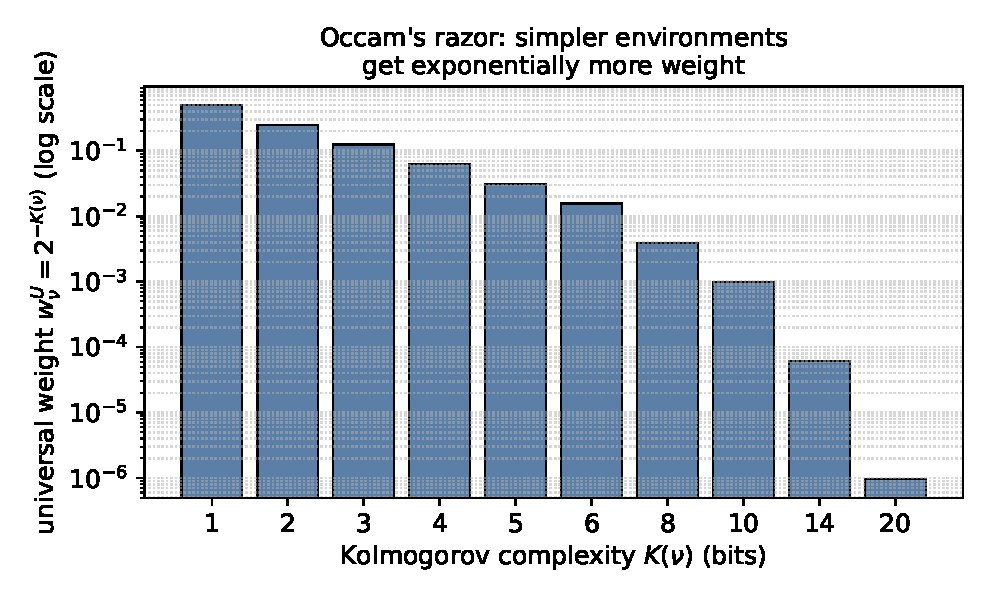
\includegraphics[width=0.62\textwidth]{universal_prior}
  \end{center}
\end{frame}

% ============================================================
\section{7.5 Exercises}

\begin{frame}[allowframebreaks]{Exercises}
  \small
  \begin{enumerate}
    \item[1.] [C15] Explicate the proof of Definition 7.2.2 by lifting the
      proof of Theorem 3.1.7.
    \item[2.] [C15] Use Blackwell \& Dubin's Theorem 3.9.5 to prove the
      agent version Theorem 7.2.6.
    \item[3.] [C21i] Complete the proof of Theorem 7.3.1.
    \item[4.] [C15i] This exercise extends Definition 3.9.1 and Example
      3.9.2 to the agent case: random variables $X_t=X_t(h_{1:\infty})$ are
      said to form a supermartingale if $\mathbf{E}[X_t|h_{<t}]\le X_{t-1}$.
      Show that $X_t := \nu(e_{1:t}\|a_{1:t})/\mu(e_{1:t}\|a_{1:t})$ in the
      proof of Lemma 7.3.4 is a $\mu^\pi$-supermartingale.
    \item[5.] [C30m] Show that $X_t$ from the previous exercise converges
      to a finite constant w.$\mu$.p.1.
    \item[6.] [C30u] Show that for every enumerable chronological
      semimeasure $\rho$ there exists a Turing machine $T$ of length
      $\ell(T)=K(\rho)+O(1)$ that computes it, i.e.\
      $\rho(h_{1:t}) = \sum_{q:T(q,a_{1:t})\to e_{1:t}}2^{-\ell(q)}$.
    \item[7.] [C20u] Let $\delta(t)=\sum_{\nu\in\Mcal}w_\nu\delta_\nu(t)$
      and $\sum_{\nu\in\Mcal}w_\nu\le1$. Show that the boundedness
      assumption $0\le\delta_\nu(t)\le c$ is necessary for $\delta_\nu(t)\to0$
      as $t\to\infty$ to imply existence and/or convergence of $\delta(t)$.
      Show that $\delta_\nu(t)=O(f(t))\ \forall\nu\in\Mcal$ does not
      necessarily imply $\delta(t)=O(f(t))$ if $\Mcal$ is infinite, even for
      bounded $\delta_\nu$.
    \item[8.] [C30ui] Consider an environmental class $\Mcal$ that admits
      self-optimizing policies. Study the effect of additionally believing
      in some $\rho\notin\Mcal$ with small probability $\alpha$ (alpha): the
      new belief prior is $\xi':=(1-\alpha)\xi+\alpha\rho$. Show that a
      belief $\alpha$ in $\rho$ much smaller than the belief $w_\mu$ in the
      true environment $\mu\in\Mcal$ only causes a small corruption of the
      self-optimizing property. More precisely, show
      $\limsup_{t\to\infty}\big[V_\mu^*(h_{<t}) - V_\mu^{\pi_{\xi'}^*}(h_{<t})\big]
      \le \frac{\alpha}{(1-\alpha)w_\mu}$.
    \item[9.] [C40o] How does AIXI perform when the sets of observations
      $\mathcal O$ and actions $\Acal$ are countably infinite? Is it still
      self-optimizing?
    \item[10.] [C35] How does AIXI perform on the sequence-prediction
      problem? When the environments consist purely of sequence-prediction
      environments, how well does AIXI do?
    \item[11.] [C10] Show that replacing the posterior $w(\nu|h_{<t})$ with
      the prior $w_\nu$ in Theorem 7.4.2 leaves the optimal action
      unaffected. Show that the ``constant'' $\xi(e_{<t}\|a_{<t})$ (7.4.6)
      can indeed be dropped from Theorem 7.4.2.
    \item[12.] [C20] Show that there exists a universal chronological
      Turing machine (Definition 7.4.4).
    \item[13.] [C20] Show that $\nu(e_{1:m}\|a_{1:m})$ (7.4.8),
      $\xi(e_{1:m}\|a_{1:m})$ (7.4.7), and $M(e_{1:m}\|a_{1:m})$ (Theorem
      7.4.5) are all chronological semimeasures.
    \item[14.] [C20] Show that there exists a universal chronological
      semimeasure (Definition 6.3.1) in the sense of dominating all other
      semicomputable chronological semimeasures, analogous to Proposition
      3.1.4.
    \item[15.] [C30] Show that $M(e_{1:m}\|a_{1:m})\stackrel{\times}{=}
      \xi_U(e_{1:m}\|a_{1:m})$ (7.4.9).
    \item[16.] [C20] Show that $M(e_{1:m}\|a_{1:m})$ is a universal
      chronological semimeasure, analogous to Proposition 3.1.4.
    \item[17.] [C40o] Derive a model-free version of AIXI, in the same way
      Q-learning is a model-free RL algorithm for MDPs.
    \item[18.] [C33] AIXI has uncertainty over its future and models this
      with $M$. What if AIXI was also uncertain about its \emph{past}? How
      would AIXI resolve this uncertainty, and what would this AIXI look
      like?
    \item[19.] [C25] How well does AIXI perform on environments not in
      $\Mcal$? \emph{Hint}: make an assumption about how close the
      environment is to an environment in $\Mcal$, possibly similar to
      Section 3.4.
  \end{enumerate}
  \small\textit{Difficulty tags} (e.g.\ [C15], [C30u]) are the book's own
  rating of roughly how hard/technical each exercise is, higher being
  harder; the trailing letters flag exercise \emph{type} (e.g.\ ``i''
  implementation-flavoured, ``u'' unsolved/open, ``o'' open research
  question).
\end{frame}

% ============================================================
\section{7.6 History and References}

\begin{frame}[allowframebreaks]{History and References}
  \textbf{Universal artificial intelligence.} The field began with
  [Hut00], which defined the agent AIXI, argued why AIXI is the most
  intelligent agent possible, showed how AIXI subsumes several interesting
  environment classes, provided a computable approximation of AIXI, and
  introduced an intelligence order relation leading to the universal
  intelligence measure $\Upsilon$ (Definition 16.7.1, later in the book).
  This work was extended into the tech report [Hut03d] and summarized in
  [Hut01e, Hut01f, Hut13b], then extended further into the book [Hut05b],
  which contains everything covered in this chapter. Further study into
  what intelligence \emph{is} and how it should be defined, measured, and
  tested appears in [LH05, LH06, LH07a, LH07c, LH07b]. Universal AI as a
  top-down approach to building artificial general intelligence is
  described in [Hut07f]; many of UAI's open problems are collected in
  [Hut09g], some since solved. An axiomatic approach [SH11a, SH11b]
  demonstrates that rational agent behaviour naturally leads to AIXI.
  [Hut12b] surveys advances since UAI's inception and future directions;
  [EH18b] is a succinct, up-to-date survey of the field. Figure 7.1's
  taxonomy, and the proofs behind it, appear in [Hut05b, LH04]; [RH06,
  RH08a] develop more general criteria for (upper) self-optimizingness,
  based on \emph{recoverable}, \emph{strongly explorable}, and
  (worst-case) \emph{value-stable} environments.

  \framebreak
  \textbf{Bayesian reinforcement learning.} UAI is a form of
  \emph{history-based} universal Bayesian reinforcement learning, though
  most of the wider Bayesian RL literature is studied within the narrower
  MDP framework; see [GMPT15] for a survey. [BVB13] shows how Bayesian
  inference can reduce the cost of learning an environment by factorizing
  the observation space, tested empirically on Atari 2600 games [BNVB13].
  [SHL97] finds an optimal policy for the maximum-a-posteriori (MAP)
  estimate of the true environment; [Str00a] takes a similar approach,
  solving for the environment with highest likelihood. [RK17] takes a
  Bayesian approach to bandits, a special case of MDPs; [OB10b] allows the
  agent to model external interventions to its own behaviour.

  \vspace{2mm}
  \textbf{Partial observability.} Most reinforcement learning is
  formulated within the MDP framework, but real agents often receive only
  limited information about the true state (\textbf{POMDPs} --- Partially
  Observable MDPs). [PVHR06] gives a Bayesian model-based POMDP solution
  and an algorithm, BEETLE, later extended to MDPs [PV08]. [RCdP07]
  approximates the space of all belief distributions over states (the
  \emph{belief space}) via a finite-dimensional subspace to obtain
  $\varepsilon$-optimal solutions; both [RCdP07, PV08] factor beliefs using
  mixtures of Dirichlet distributions. [WLBS05] uses ``sparse sampling'' to
  approximate Bayes-optimal decision making. POTMMCP [SKH23] is an
  online MCTS-based planner for large POMDPs with good theoretical
  guarantees and practical performance in multi-agent settings. A
  heuristic market-based RL algorithm [Bau99, Bau04] --- where reward is a
  conserved, scarce currency agents pay and receive for services --- has
  been evaluated in POMDP environments in [KHS01b].

  \framebreak
  \textbf{Causality.} This book does not explicitly consider causality,
  which may be surprising. The actions and percepts in a history
  $h_{1:\infty}=a_1e_1a_2e_2\dots$ have a clear temporal order, and the
  chronology condition (Definition 6.3.1) already ensures actions and
  percepts only ever depend on the past, never the future --- which is all
  the causal structure this book needs. There are of course deeper research
  questions requiring a more explicit treatment of causality [Pea00, PGJ16,
  PM18, PJS17] within Universal AI [OKD+21, EHKK21, CVH21, EKH19, EH18a,
  ELH15] and beyond [HH22]; for instance, [MWV+21] studies the difficult
  \emph{credit assignment} problem of determining an action's influence on
  future rewards from a counterfactual point of view.
\end{frame}

% ============================================================
\begin{frame}{Summary: Chapter 7}
  \begin{itemize}
    \item \textbf{AI$\mu$} (Sec.\ 7.1) is the fully-informed optimal agent:
      given the true environment $\mu$, its action at every step is the
      $\arg\max$/expectation \textbf{expectimax} tree of Proposition 7.1.2,
      truncated to a finite horizon and approximated in practice via
      pruning, learned heuristics, or Monte Carlo Tree Search.
    \item The \textbf{Bayes mixture} $\xi=\sum_\nu w_\nu\nu$ (Def.\ 7.2.1)
      combines a whole class $\Mcal$ of candidate environments into one
      known distribution, whose posterior weights $w(\nu|h_{<t})$ update via
      Bayes' rule (Def.\ 7.2.2) exactly as in Chapter 3, now conditioned on
      actions too.
    \item \textbf{Merging of opinions} (Thm.\ 7.2.6) and \textbf{on-policy
      value convergence} (Thm.\ 7.3.1) show $\xi\to\mu$ and $V_\xi\to V_\mu$
      in a strong sense, with no i.i.d.\ or stationarity assumptions.
    \item \textbf{AI$\xi$} (Def.\ 7.3.2) plans against its current belief
      $\xi$ instead of the unknown $\mu$; it is \textbf{self-optimizing}
      (Thm.\ 7.3.6) for any class $\Mcal$ that admits \emph{some}
      self-optimizing policy --- but self-optimizing fails in general due to
      irrecoverable \textbf{traps} (Figure 7.1).
    \item \textbf{AIXI} (Def.\ 7.4.1) specializes $\Mcal$ to \emph{every}
      computable environment and $w_\nu$ to the \textbf{universal prior}
      $2^{-K(\nu)}$, giving the most environment-independent Bayesian agent
      conceivable, with an equivalent \textbf{Solomonoff/Turing-machine}
      formulation (Thm.\ 7.4.5) and a guarantee that it is never fooled into
      pessimism in genuinely good environments (Thm.\ 7.4.10).
    \item Chapter 8 next develops weaker, on-average optimality notions
      that work even where self-optimizing policies do not exist.
  \end{itemize}
\end{frame}

\end{document}
